% ----- formatovani dokumentu -----------------------------------------------
\documentclass[12pt,a4paper,titlepage,final]{report}
\usepackage[utf8]{inputenc}
\usepackage[T1, IL2]{fontenc}
\usepackage{graphicx}
\usepackage{epstopdf}
\usepackage[margin=2cm]{caption}
\usepackage[top=3cm, left=2cm, right=2cm, text={17cm, 24cm}, ignorefoot]{geometry}
\usepackage{color}
\usepackage{url}
\usepackage{setspace}
\usepackage{amsmath}
\usepackage{xcolor}
\singlespacing
\usepackage[square, numbers]{natbib}
\pagestyle{plain}
\pagenumbering{arabic}
\setcounter{page}{1}
\setcounter{secnumdepth}{-1}
\setlength{\parindent}{1cm}
\usepackage{natbib}


% ----- vyberte jazyk -------------------------------------------------------
\usepackage[english,czech]{babel}
%\usepackage[english]{babel}

% ----- dopiste titulky -----------------------------------------------------
\newcommand\Course{Počítačová grafika}
\newcommand\WorkTitle{Generátor kinetické typografie}
\newcommand\AuthorA{Jan Hrdina}
\newcommand\AuthorAEmail{xhrdin10@stud.fit.vutbr.cz}
\newcommand\AuthorB{Peter Gazdík}
\newcommand\AuthorBEmail{xgazdi03@stud.fit.vutbr.cz}
\newcommand\Faculty{Fakulta Informačních Technologií}
\newcommand\School{Vysoké Učení Technické v Brně}

\usepackage[
pdftitle={\WorkTitle},
pdfauthor={\AuthorA, \AuthorB},
bookmarks=true,
colorlinks=true,
breaklinks=true,
urlcolor=blue,
citecolor=blue,
linkcolor=blue,
unicode=true,
]
{hyperref}


% ----- titulni strana ------------------------------------------------------

\begin{document}
	\begin{titlepage}
	\begin{center}
		
\includegraphics[width=14cm]{images/logo.eps}
	\end{center}
	\vfill
	\begin{center}
		\begin{Large}
			\Course\\
		\end{Large}
		\bigskip
		\begin{Huge}
			\WorkTitle\\
		\end{Huge}
	\end{center}
	\vfill
	\begin{center}
		\begin{large}
			\today
		\end{large}
	\end{center}
	\vfill
	\begin{flushleft}
		\begin{large}
			\begin{tabular}{lll}
				Autoři: & \AuthorA, & \url{\AuthorAEmail} \\
				        & \AuthorB, & \url{\AuthorBEmail} \\
				& & \\
				& \Faculty \\
				& \School \\
			\end{tabular}
		\end{large}
	\end{flushleft}
\end{titlepage}

% ----- obsah --------------------------------------------------------------

%\tableofcontents

% ----- zadani -------------------------------------------------------------
\newpage
\chapter{Zadání}

\begin{itemize}
\item Uživatel při spuštění aplikaci předá soubor s libovolným textem
\item Aplikace postupně text zobrazí
  \begin{itemize}
  \item animovaně s nelineárními časovými křivkami (Beziérovy kubiky)
  \item ve 3D
  \item vhodně esteticky rozdělený a rozmístěný
  \end{itemize}
\item Aplikace náhodně vybírá z možných animačních efektů a uspořádání
  \begin{itemize}
  \item Každý efekt si může klást různé požadavky na čtený text, např. \uv{začíná čtyřmi slovy, z nichž první je krátké a druhé je středně dlouhé}
  \item Podle vhodnosti efektu pro zbývající text je efektu přiřazena váha, která ovlivňuje pravděpodobnost vybrání.
  \end{itemize}
\end{itemize}

%Zde napište informace k zadání (nejde jen o přepis toho, co je na webu;
%komentujte vaše vlastní zpřesnění zadání, zaměření, důrazy, pojetí atd.). Text
%strukturujte, použijte odrážky, číslování$\ldots$

%\paragraph{Rozsah:} cca 10 odrážek

%---------------------------------------------------------------------------
\chapter{Použité technologie}

\begin{itemize}

\item GLEW
\item GLFW
\item FTGL - Knihovna pro vykreslování textu v OpenGL - neoficiální verze přidávající podporu OpenGL 3 dostupná na \url{https://github.com/lukexi/ftgl3}
\end{itemize}

%Zde vypište, jaké technologie vaše řešení používá – co potřebuje k běhu, co jste použili při tvorbě, atd. Text strukturujte, použijte odrážky, číslování \dots

%\paragraph{Rozsah:} cca 7 odrážek


%---------------------------------------------------------------------------
\chapter{Použité zdroje}

\begin{itemize}
\item Beziérovy kubiky \cite{bezier}
\item OpenGL tutorial \cite{learnopengl}
\item Fonty + licence
\begin{itemize}
\item Roboto -- Apache License, Version 2.0
\item Fira Mono -- Open Font License, Version 1.1
\item DejaVuSerif -- licence viz \url{http://dejavu-fonts.org/wiki/License}
\end{itemize}
\item Texty
\begin{itemize}
\item demos/dream - Martin Luther King, Jr., I Have a Dream \cite{speech:dream}
\item demos/havel - První novoroční projev Václava Havla \cite{speech:havel}
\end{itemize}
\item Videa s kinetickou typografií \cite{video:soe} \cite{video:kity}
\item Open-source herný engine Cocos2d-x \cite{cocos}
\item Kniha Game programming patterns \cite{patterns}
\end{itemize}  

%Zde vypište, které zdroje jste použili k tvorbě: hotový kód, hotová data (obrázky, modely, \dots), studijní materiály. Pokud vyplyne, že v projektu je použit kód nebo data, která nejsou uvedena tady, jedná se o závažný problém a projekt bude pravděpodobně hodnocen 0 body.

%\paragraph{Rozsah:} potřebný počet odrážek

%---------------------------------------------------------------------------
\chapter{Nejdůležitější dosažené výsledky}

\section{Estetika}

Při návrhu efektů a podpůrných tříd jsme si dali záležet na výsledných estetických kvalitách.

\begin{itemize}
	\item Využíváme nelineárních animačních křivek
    \item Snažili jsme se pečlivě volit kompozici textu, podpůrné metody kreslení textu umožňují neobvyklé požadavky jako \uv{Automaticky nastav velikost písma tak aby šířka textu byla pokud možno přesně 600px a zároveň jeho výška nepřesáhla 800px}
    \item Volba vhodného efektu pro aktuální text - když například text začíná krátkým slovem, je větší pravděpodobnost, že se vybere efekt který toho dokáže využít a například zarovnat velké \uv{I} po straně řádků \uv{I have a dream}
\end{itemize}

\begin{center}
	\captionsetup{type=figure}
		
\includegraphics[width=10cm]{images/dream.png}
	\captionof{figure}{Efekt \uv{LetterAside}}
\end{center}

\section{Kompletní animační framework}

Pro zajištění snadné manipulace s textovými objekty jsme vytvořili 3D animační framework. Při jeho implementování jsme se inspirovali 2D herním enginem cocos2d-x\cite{cocos} a návrhovými vzory publikovanými v knize Game Programming Patterns \cite{patterns}.

\begin{itemize}
	\item Animace v čase -- posuny, rotace, škálování, změna průhlednosti.
    \item Seskupování animací do skupin a jejich paralelní / sekvenční vykonávání.
    \item Invokace vlastních funkcí v průběhu vykonávání animací.
    \item Úprava časového průběhu animací pomocí beziérových kubik\cite{bezier}.
    \item Pozicování nezávislé na velikosti okna.
    \item Pozicování objektů relativně k jejich rodičovskému objektu v grafu scény a seskupování objektů.
\end{itemize}


\section{Snadné přidávání nových efektů}

Vše je navrženo tak, aby bylo možné snadno přidávat nové efekty. Pro maximální usnadnění této činnosti jsme dokonce vytvořili skript genEffect, který vytvoří šablonu pro efekt se zadaným názvem a rovnou jej zaregistruje v aplikaci.


%---------------------------------------------------------------------------
\chapter{Zvláštní použité znalosti} \label{znalosti}

\section{Rotace kolem pivotu}

Aby bylo možné rotovat objekty v jiném bodě, než je jejich počátek (v tzv. pivotu), je potřeba před vykonáním rotace upravit pozici počátku na základě pozice pivotu. Nejjednodušší způsob, jak tohoto docílit je před samotnou rotací posunout celý objekt do tohoto bodu, vykonat rotaci a následně celý objekt posunout zpět. Toto má však za následek narušení relativního pozicování ostatních objektů, které jsou potomky aktuálního objektu.

Abychom se tomu vyhnuli, je potřeba upravit pozici počátku na základě hodnoty aktuální rotace a pozice pivotu a ne jen na základě pozice pivotu. K aktuální pozici tedy potřebujeme připočítat hodnotu danou následujícím výpočtem, kde matice odpovídá transformační matici rotace postupně v osách $x$, $y$ a $z$ a body $x$, $y$ a $z$ představují pozici pivotu.

\begin{equation*}
\begin{bmatrix} 
{\cos \beta \cos \gamma} & {-\cos \beta \sin \gamma } & {\sin \beta} & 0 \\ 
{\cos \alpha \sin \gamma + \sin \alpha \sin \beta \cos \gamma } & {\cos \alpha \cos \gamma - \sin \alpha \sin \beta \sin \gamma } & - {\sin \alpha \cos \beta} & 0 \\ 
{\sin \alpha \sin \gamma - \cos \alpha \sin \beta \cos \gamma} & {\sin \alpha \cos \gamma + \cos \alpha \sin \beta \sin \gamma} & {\cos \alpha \cos \beta} & 0 \\ 
0 & 0 & 0 & 1 \end{bmatrix} 
\cdot ({-1}) 
\cdot 
\begin{pmatrix} 
x \\ y \\ z \\ 1 
\end{pmatrix}
\end{equation*}

\section{Úprava časového průběhu animací}

Pro dosažení přirozeného vzhledu jednotlivých akcí animační framework umožňuje upravit jejich jinak lineární časový průběh. Nový časový průběh je parametrizovatelný pomocí Beziérovy křivky, která je definovaná čtveřicí bodů, viz obrázek \ref{fig:bezier}. Algoritmus výpočtu Beziérovy kubiky je převzat z článku Bezier Curve based easing functions\cite{bezier}.

\begin{figure}
\begin{center}
		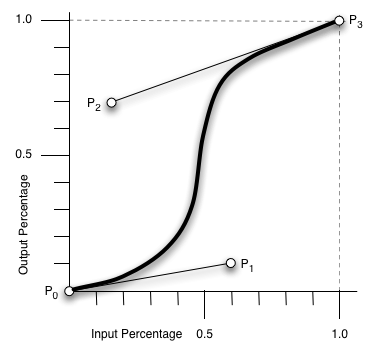
\includegraphics[width=7.5cm]{images/timing-function.png}
	\caption{Časový průběh definovaný čtveřicí hodnot $P_0-P_3$\cite{bezier}}
    \label{fig:bezier}
\end{center}
\end{figure}


\section{DoF a motion blur v OpenGL 3}

Původně jsme plánovali do projektu začlenit podporu depth-of-field a motion blur. Oba algoritmy se dají snadno realizovat s využitím Accumulator Bufferu, proto jsme si jejich implementaci nechali až nakonec. Bohužel se nicméně pár dní před odevzdáním ukázalo, že accumulator buffer je od OpenGL v3.2 odstraněn z Core Profile \cite{opengl} a je tedy nutné buďto využít Compatibility Profile, který nám nefungoval s FTGL, nebo využít jiných prostředků.

Pro DoF je například možné využít vlastních FBO, kdy se obrazová a hloubková složka rasterizované scény vyrenderují do textury, která se následně zpracovává ve fragment shaderu. Dá se tak dosáhnout zajímavých výsledků (viz \cite{blog:dof}), nicméně z časových důvodů jsme tuto náročnější implementaci již nestihli. Podstatné je, že po tomto kurzu už to pro nás není španělská vesnice a kdybychom měli pár dní navíc, určitě bychom to zvládli.

\section{Ladění OpenGL}

Při ladění jsme si vyzkoušeli práci s nástrojem Intel Graphics Performance Analyzer, který umožňuje analyzovat stav pipeline OpenGL v čase, debugovat shadery a dokonce i rozebírat jednotlivé objekty ve scéně. Program je dostupný na \url{https://software.intel.com/en-us/gpa}

\section{Náhodný výběr prvků z pole s vahami}

Při náhodném výběru textového efektu využíváme algoritmus zohledňující váhy jednotlivých efektů. Algoritmus jsme převzali z \url{http://softwareengineering.stackexchange.com/a/150678}

\section{Techniky vykreslování textu}

Pro naši realizaci bylo přirozeně nutné nastudovat způsoby řešení vykreslování textů pomocí OpenGL.

Metody pracují většinou na jednom ze dvou principů:

\begin{itemize}
\item \textbf{Text jako bitmapa} -- text se mimo OpenGL vykreslí do bitmapy a ta je následně v OpenGL použita jako textura. Přístupy se můžou lišit podle toho, jestli se vytvoří bitmapa se všemi glyphy a z nich se pak skládají řetězce nebo se renderuje každý řetězec zvlášť
\item \textbf{Text jako vektor} -- text se pomocí tesselátoru převede z polygonálního popisu na trojúhelníky a ty se rasterizují již pomocí grafické karty. Tuto metodu využíváme my.
\end{itemize}

Pro načítání fontů a jejich polygonální reprezentace slouží knihovna FreeType. O podporu tesselace, pozicování a použití v OpenGL ji doplňuje knihovna FTGL, kterou využíváme. Původní knihovna FTGL s poslední aktualizací v roce 2011 bohužel nepodporuje OpenGL 3, proto jsme použili neoficiální fork.

%Uveďte informace, které byly potřeba nad rámec výuky probírané na FIT.
%Vysvětlete je pomocí obrázků, schémat, vzorců apod.

%\paragraph{Rozsah:} podle potřeby a vlastního uvážení


%---------------------------------------------------------------------------
\chapter{Práce na projektu}

\section{Rozdělení práce v týmu}

\begin{itemize}
\item \textbf{\AuthorA}: Implementace efektů, vykreslování/pozicování textů, celková vize
\item \textbf{\AuthorB}: Animační engine (animace, akce, graf scény, vykreslování, \dots)
\end{itemize}

%---------------------------------------------------------------------------
\section{Co bylo nejpracnější}

\begin{itemize}
\item \textbf{\AuthorA}
	\begin{itemize}
    \item Pozicování a transformace textu v souřadném systému u efektů a vytvoření vhodných abstrakcí
    \item Koordinace a návaznost animací
    \end{itemize}
\item \textbf{\AuthorB}:
\begin{itemize}
	\item Přechod na FTGL s podporou OpenGL 3.0
	\item Pokročilejší transformace vyžadující znalosti lineární algebry.
    \item Vytvoření souřadného systému simulujícího ortogonální projekci pro zabezpečení jednoduchého pozicování.
\end{itemize}
\end{itemize}

%---------------------------------------------------------------------------
\section{Zkušenosti získané řešením projektu}

\begin{itemize}
\item Trello a Scrum se opět osvědčily na organizaci a plánování vývoje
\item Overleaf na online psaní dokumentace
\item Osvojení nových technologií a dovedností, viz \nameref{znalosti}
\end{itemize}

---------------------------------------------------------------------------
\chapter{Autoevaluace}

\paragraph{Technický návrh (80\%):} (analýza, dekompozice problému, volba
vhodných prostředků, $\ldots$)

  \begin{itemize}
  \item Návrh architektury pomocí UML diagramu tříd
  \item oddělení OpenGL detailů od zbytku aplikace
  \item odstínění kódu efektů od implementačních detailů
  \end{itemize}

\paragraph{Programování (70\%):} (kvalita a čitelnost kódu, spolehlivost běhu,
obecnost řešení, znovupoužitelnost, $\ldots$)

  \begin{itemize}
  \item Snaha o intuitivní názvy identifikátorů
  \item Využití C++11 a moderních konstrukcí
  \end{itemize}

\paragraph{Vzhled vytvořeného řešení (80\%):} (uvěřitelnost zobrazení,
estetická kvalita, vhled GUI, $\ldots$)

  \begin{itemize}
  \item Pravidlo třetin v kompozici
  \item Pečlivá typografie
  \item Easing
  \end{itemize}

\paragraph{Využití zdrojů (90\%):} (využití existujícího kódu a dat, využití
literatury, $\ldots$)

  \begin{itemize}
  \item Architektura inspirovaná 2D herním enginem cocos2d-x
  \item Návrhové vzory uvedené v elektronické verzi knihy Game Programming
  \end{itemize}

\paragraph{Hospodaření s časem (90\%):} (rovnoměrné dotažení částí projektu,
míra spěchu, chybějící části řešení, $\ldots$)

  \begin{itemize}
  \item Práce na projektu v čase rozložena rovnoměrně
  \item Absence pokročilejších post-processing efektů - nechali jsme je na poslední chvíli, protože jsme spoléhali na jednoduchou implementaci pomocí accumulator bufferu, který, jak se ukázalo, již není podporován. Prozkoumali jsme techniky implementace v současných API, ale z důvodu nečekané časové náročnosti jsme ji vynechali.
  \end{itemize}

\paragraph{Spolupráce v týmu (100\%):} (komunikace, dodržování dohod, vzájemné
spolehnutí, rovnoměrnost, $\ldots$)

  \begin{itemize}
  \item Využití Gitu, Trella, Skype, chatu
  \item Rychlá komunikace v obou směrech
  \end{itemize}

\paragraph{Celkový dojem (87\%):} (pracnost, získané dovednosti, užitečnost,
volba zadání, cokoliv, $\ldots$)

Bavilo a motivovalo nás pracovat na vlastním zadání, bylo osvěžující pracovat na aplikaci čistě pro estetický požitek.
Jsme rádi, že jsme si mohli osahat OpenGL, ke kterému by se člověk jinak nejspíš těžko nutil. Pracovali jsme tvrdě, ale výsledek (myslíme) stálo za to.

%---------------------------------------------------------------------------
\chapter{Ovládání vytvořeného programu}

\section{Technologie potřebné pro spuštění programu}

\begin{itemize}
    \item cmake
	\item GLEW
    \item GLFW
    \item FTGL
    \item GLM
\end{itemize}

\section{Obsluha programu}

Aplikace se spouští v příkazovém řádku. Přijímá minimálně jeden parametr - cestu k souboru se vstupním textem. Volitelně je možné s parametrem \texttt{-s} předat číselný seed pro generátor pseudonáhodné posloupnosti efektů.

Příklady spuštění aplikace:

\begin{itemize}
	\item ./pgr-project demos/dream
  	\item ./pgr-project -s 42 demos/dream
\end{itemize}

Před začátkem animace jsme přidali 4sekundovou prodlevu pro možnost zvětšit okno na celou obrazovku apod.

%---------------------------------------------------------------------------
\chapter{Doporučení pro budoucí zadávání projektů}

Oceňujeme možnost realizace vlastního tématu. Na organizaci bychom nic neměnili.

%---------------------------------------------------------------------------

\bibliographystyle{plain}

\nocite{patterns}
\nocite{cocos}
\nocite{wiki:dof}
\nocite{wiki:mb}
\nocite{video:kity}
\nocite{video:soe}

\bibliography{reference}
\addcontentsline{toc}{chapter}{Literatura}

\end{document}
